% debugging/debugging.tex

\QuickQuizChapter{chp:Validation}{Validation}

I have had a few parallel programs work the first time, but that is only
because I have written so many parallel programs over the past two decades.
And I have had far more parallel programs that fooled me into thinking
that they were working correctly the first time than actually were working
the first time.

I have therefore had great need of validation for my parallel programs.
The basic trick behind parallel validation, as with other software
validation, is to realize that the computer knows what is wrong.
It is therefore your job to force it to tell you.

@@@ roadmap

\section{Tracing}
\label{sec:debugging:Tracing}

\section{Assertions}
\label{sec:debugging:Assertions}

\section{Static Analysis}
\label{sec:debugging:Static Analysis}

\section{Probability and Heisenbugs}
\label{sec:analysis:Probability and Heisenbugs}

So your parallel program fails.
Sometimes.

But you figured out the problem and now have a fix in place!
Congratulations!!!

But now how much testing do you have to do in order to be certain that
you actually fixed the bug, as opposed to just reducing the probability
of it occurring on the one hand or having fixed only one of several
related bugs on the other?

Unfortunately, the honest answer is that an infinite amount of testing
is required to attain absolute certainty.

\QuickQuiz{}
	Suppose that you had a very large number of systems at your
	disposal.
	For example, at current cloud prices, you can purchase a
	huge amount of CPU time at a reasonably low cost.
	Why not use this approach to get close enough to certainty
	for all practical purposes?
\QuickQuizAnswer{
	This approach might well be a valuable addition to your
	validation arsenal.
	But it does have a few limitations:
	\begin{enumerate}
	\item	Some bugs have extremely low probabilities of occurrence,
		but nevertheless need to be fixed.
		For example, suppose that the Linux kernel's RCU
		implementation had a bug that is triggered only once
		per century of machine time on average.
		A century of CPU time is hugely expensive even on
		the cheapest cloud platforms, but we could expect
		this bug to result in more than 2,000 failures per day
		on the more than 100 million Linux instances in the
		world as of 2011.
	\item	The bug might well have zero probability of occurrence
		on your test setup, which means that you won't see it
		no matter how much machine time you burn testing it.
	\end{enumerate}
	Of course, if your code is small enough, formal validation
	may be helpful, as discussed in
	Appendix~\ref{app:formal:Formal Verification}.
} \QuickQuizEnd

But suppose that we are willing to give up absolute certainty in favor
of high probability.
Then we can bring powerful statistical tools to bear on this problem.
However, this section will focus on simple statistical tools.
These tools are extremely helpful, but readers should not make the
mistake of assuming that reading this section is in any way a substitute
for taking a good set of statistics classes.\footnote{
	Which I most highly recommend.
	The few statistics courses I have taken have provided value
	way out of proportion to the time I spent studying for them.}

For our start with simple statistical tools, we need to decide whether
we are doing discrete or continuous testing.
Discrete testing features well-defined individual test runs.
For example, a boot-up test of a Linux kernel patch is an example
of a discrete test.
You boot the kernel, and it either comes up or it does not.
Although you might spend an hour boot-testing your kernel, the number of
times you attempted to boot the kernel and the number of times the
boot-up succeeded would often be of more interest than the length
of time you spent testing.
Functional tests tend to be discrete.

On the other hand, if my patch involved RCU, I would probably run
rcutorture, which is a kernel module that, strangely enough, tests RCU.
Unlike booting the kernel, where the appearance of a login prompt
signals the successful end of a discrete test, rcutorture will happily
continue torturing RCU until either the kernel crashes or until you
tell it to stop.
The duration of the rcutorture test is therefore (usually) of more
interest than the number of times you started and stopped it.
Therefore, rcutorture is an example of a continuous test, a category
that includes many stress tests.

The statistics governing discrete and continuous tests differs somewhat.
However, the statistics for discrete tests is simpler and more
familiar than that for continuous tests, and furthermore the
statistics for discrete tests can often be pressed into service
(with some loss of accuracy) for continuous tests, we start with
discrete tests.

\subsection{Statistics for Discrete Testing}
\label{sec:Statistics for Discrete Testing}

Suppose that the bug had a 10\% chance of occurring in
a given run and that we do five runs.
How do we compute that probability of at least one run failing?
One way is as follows:

\begin{enumerate}
\item	Compute the probability of a given run succeeding, which is 90\%.
\item	Compute the probability of all five runs succeeding, which
	is 0.9 raised to the fifth power, or about 59\%.
\item	There are only two possibilities: either all five runs succeed,
	or at least one fails.
	Therefore, the probability of at least one failure is
	59\% taken away from 100\%, or 41\%.
\end{enumerate}

However, many people find it easier to work with a formula than a series
of steps, although if you prefer the above series of steps, have at it!
For those who like formulas, call the probability of a single failure $f$.
The probability of a single success is then $1-f$ and the probability
that all of $n$ tests will succeed is then:

\begin{equation}
	S_n = \left(1-f\right)^n
\end{equation}

The probability of failure is $1-S_n$, or:

\begin{equation}
	F_n = 1-\left(1-f\right)^n
\label{eq:debugging:Binomial Failure Rate}
\end{equation}

\QuickQuiz{}
	Say what???
	When I plug the earlier example of five tests each with a
	10\% failure rate into the formula, I get 59,050\% and that
	just doesn't make sense!!!
\QuickQuizAnswer{
	You are right, that makes no sense at all.

	Remember that a probability is a number between zero and one,
	so that you need to divide a percentage by 100 to get a
	probability.
	So 10\% is a probability of 0.1, which gets a probability
	of 0.4095, which rounds to 41\%, which quite sensibly
	matches the earlier result.
} \QuickQuizEnd

So suppose that a given test has been failing 10\% of the time.
How many times do you have to run the test to be 99\% sure that
your supposed fix has actually improved matters?

Another way to ask this question is ``how many times would we need
to run the test to cause the probability of failure to rise above 99\%?''
After all, if we were to run the test enough times that the probability
of seeing at least one failure becomes 99\%, if there are no failures,
there is only 1\% probability of this being due to dumb luck.
And if we plug $f=0.1$ into 
Equation~\ref{eq:debugging:Binomial Failure Rate} and vary $n$,
we find that 43 runs gives us a 98.92\% chance of at least one test failing
given the original 10\% per-test failure rate,
while 44 runs gives us a 99.03\% chance of at least one test failing.
So if we run the test on our fix 44 times and see no failures, there
is a 99\% probability that our fix was actually a real improvement.

But repeatedly plugging numbers into
Equation~\ref{eq:debugging:Binomial Failure Rate}
can get tedious, so let's solve for $n$:

\begin{eqnarray}
	F_n = 1-\left(1-f\right)^n \\
	1 - F_n = \left(1-f\right)^n \\
	\log \left(1 - F_n\right) = n \; \log \left(1 - f\right) \\
\end{eqnarray}

Finally the number of tests required is given by:

\begin{equation}
	n = \frac{\log\left(1 - F_n\right)}{\log\left(1 - f\right)}
\label{eq:debugging:Binomial Number of Tests Required}
\end{equation}

\QuickQuiz{}
	In Equation~\ref{eq:debugging:Binomial Number of Tests Required},
	are the logarithms base-10, base-2, or base-$e$?
\QuickQuizAnswer{
	It does not matter.
	You will get the same answer no matter what base of logarithms
	you use because the result is a pure ratio of logarithms.
	The only constraint is that you use the same base for both
	the numerator and the denominator.
} \QuickQuizEnd

\begin{figure}[tb]
\begin{center}
\resizebox{3in}{!}{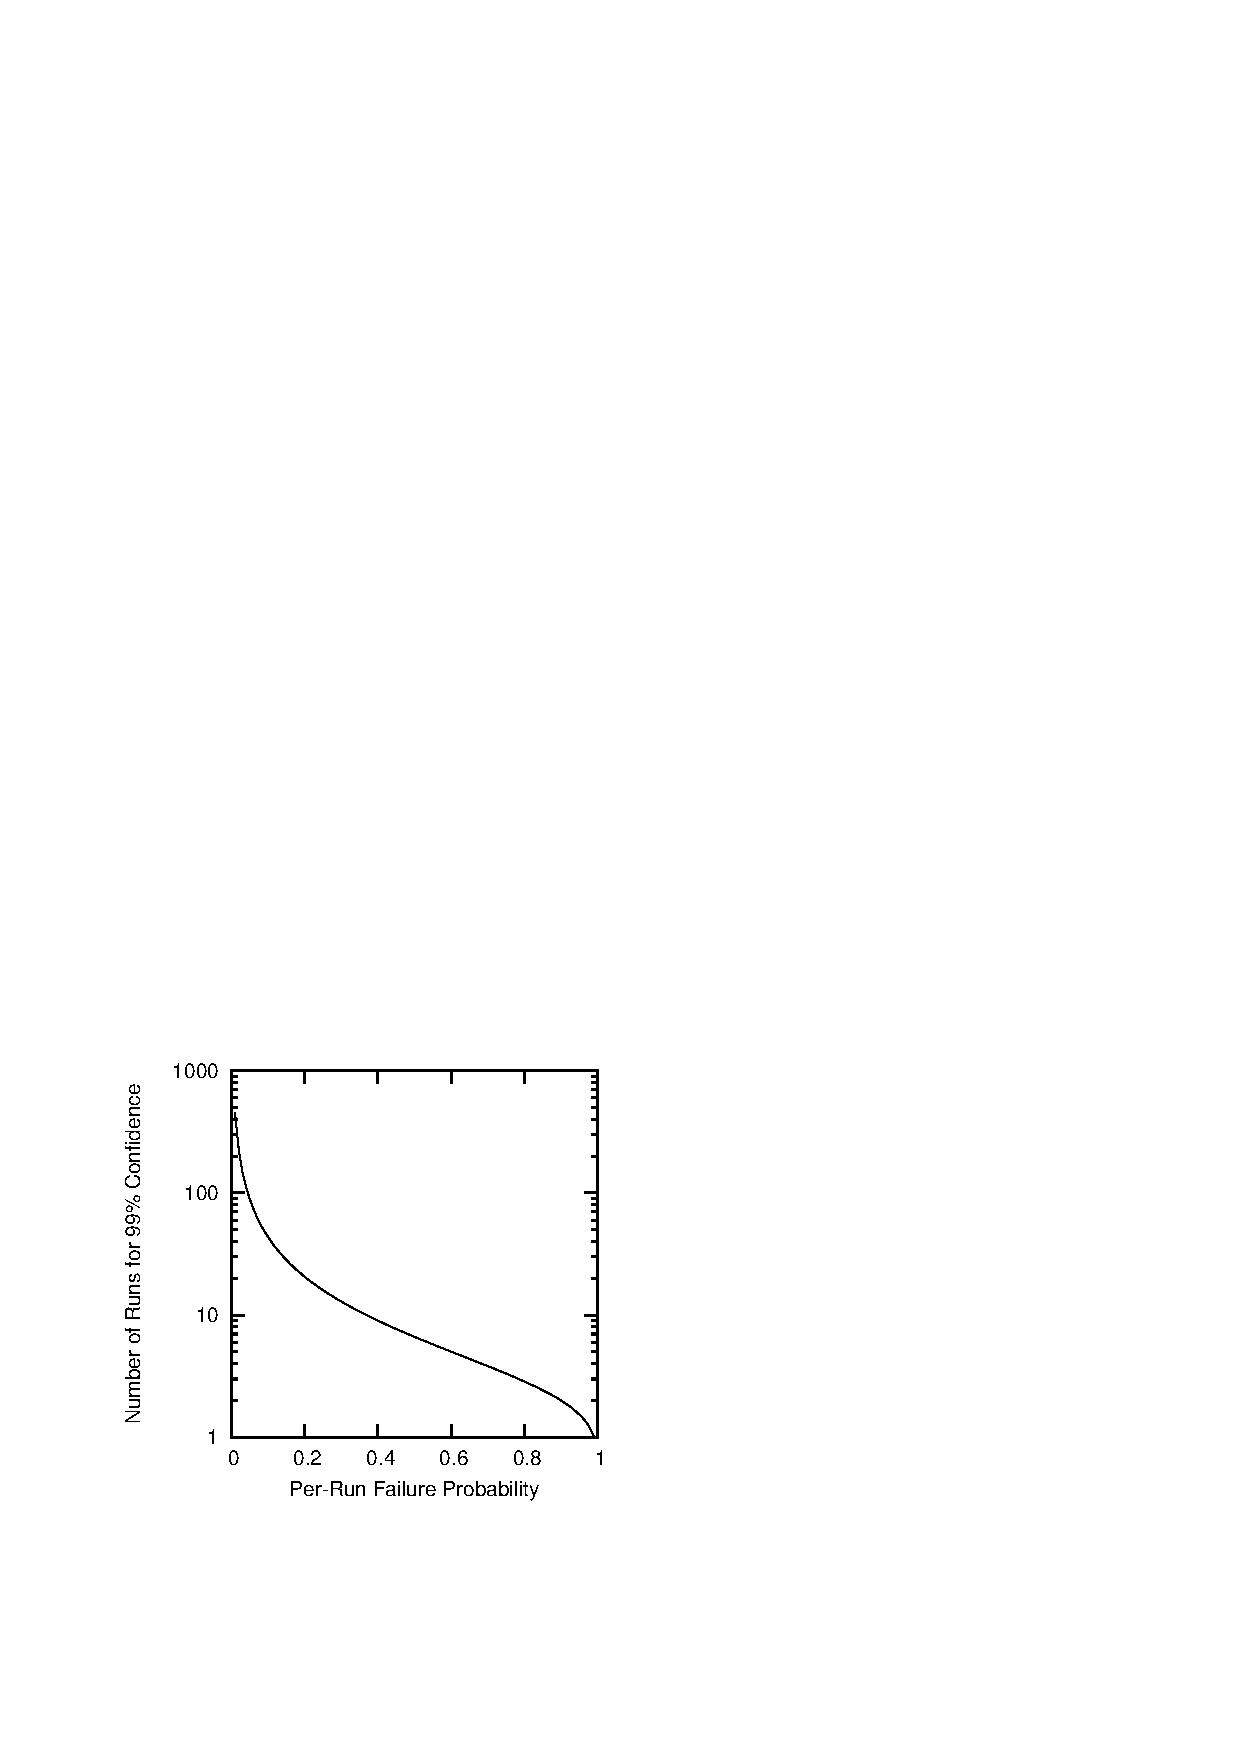
\includegraphics{CodeSamples/debugging/BinomialNRuns}}
\end{center}
\caption{Number of Tests Required for 99 Percent Confidence Given Failure Rate}
\label{fig:debugging:Number of Tests Required for 99 Percent Confidence Given Failure Rate}
\end{figure}

Figure~\ref{fig:debugging:Number of Tests Required for 99 Percent Confidence Given Failure Rate}
shows a plot of this function.
Not surprisingly, the less frequently each test run fails, the more
test runs are required to be 99\% confident that the bug has been
fixed.
If the bug caused the test to fail only 1\% of the time, then a
mind-boggling 458 test runs are required.

The moral of this story is that when you have found a rarely occurring
bug, your testing job will be much easier if you can come up with
a carefully targeted test with a much higher failure rate.
For example, if your targeted test raised the failure rate from 1\%
to 30\%, then the number of runs required for 99\% confidence
would drop from a mind-boggling 458 test runs to a mere thirteen test runs.

But these thirteen test runs would only give you 99\% confidence that
your fix had produced ``some improvement''.
Suppose you instead want to have 99\% confidence that your fix reduced
the failure rate by an order of magnitude.
How many failure-free test runs are required?

An order of magnitude improvement from a 30\% failure rate would be
a 3\% failure rate.
Plugging these numbers into
Equation~\ref{eq:debugging:Binomial Number of Tests Required} yields:

\begin{equation}
	n = \frac{\log\left(1 - 0.99\right)}{\log\left(1 - 0.03\right)} = 151.2
\end{equation}

So our order of magnitude improvement requires roughly an order of
magnitude more testing.
Certainty is impossible, and high probabilities are quite expensive.
Clearly making tests run more quickly and making failures more probable
are essential skills in the development of highly reliable software.
These skills will be covered in a later section.

\subsection{Abusing Statistics for Discrete Testing}
\label{sec:Abusing Statistics for Discrete Testing}

But suppose that you have a continuous test that fails about three
times every ten hours, and that you fix the bug that you believe was
causing the failure.
How long do you have to run this test without failure to be 99\% certain
that you reduced the probability of failure?

Without doing excessive violence to statistics, we could simply
redefine a one-hour run to be a discrete test that has a 30\%
probability of failure.
Then the results of in the previous section tell us that if the test
runs for 13 hours without failure, there is a 99\% probability that
our fix actually improved the program's reliability.

A dogmatic statistician might not approve of this approach, but the
sad fact is that the errors introduced by this sort of abuse of
statistical methodology are usually way down in the noise compared to the
errors inherent in your measurements of your program's failure rates.
Nevertheless, the next section describes a slightly less dodgy approach.

\subsection{Statistics for Continuous Testing}
\label{sec:Statistics for Continuous Testing}

@@@ continuous formulation for time-based tests leads to Poisson distribution.
This can be handled using maxima with \co{quantile_poisson()} and
\co{cdf_poisson()}, after a \co{load(distrib)}.

\subsection{Heisenbugs and Creating Anti-Heisenbugs}
\label{Heisenbugs and Creating Anti-Heisenbugs}

This line of thought also leads to an understanding of heisenbugs:
adding tracing and assertions can easily \emph{reduce} the probability
of a bug appearing.
And this is why extremely lightweight tracing and assertion mechanism are
so critically important.

\section{Profiling}
\label{sec:analysis:Profiling}

\section{Differential Profiling}
\label{sec:analysis:Differential Profiling}

{\em @@@ pull in concepts and methods from
\url{http://www.rdrop.com/users/paulmck/scalability/paper/profiling.2002.06.04.pdf}.
Also need tools work.}

\section{Performance Estimation}
\label{sec:analysis:Performance Estimation}

{\em @@@ pull in concepts and methods from
\url{http://www.rdrop.com/users/paulmck/scalability/paper/lockperf_J_DS.2002.05.22b.pdf}.}
